\chapter{Clean Architecture}

Dieses Kapitel beschreibt die Architektur der entwickelten Software. Es wurde nach den in der Vorlesung erläuterten Clean-Architecture-Prinzipien gebaut. Clean Architecture ist ein Softwarearchitektur-Muster, welches zum Ziel hat, die Abhängigkeiten innerhalb einer Anwendung zu minimieren und die Wiederverwendbarkeit und Testbarkeit zu maximieren. Es besteht aus einer inneren Schicht von unabhängigen Entitäten, die von einer äußeren Schicht von Abhängigkeiten umgeben sind. Dies ermöglicht es Entwicklern, Anwendungen zu erstellen, die leicht zu testen, zu verstehen und zu warten sind und die flexibel sind, um schnell auf Änderungen reagieren zu können.

Im Folgenden werden die verwendeten Schichten genauer erläutert. Die Schicht \enquote{Abstraction Code} wurde in unserer Anwendung nicht verwendet, da für die in der Domäne behandelten Themengebiete kein Domänen übergreifendes Wissen notwendig war, welches Teil dieser Schicht hätte sein müssen. 
Außerdem haben wir die Adapters Code Schicht und die Application Code Schicht zusammengelegt. Der Code dieser Schichten befinden sich in der Schicht 1: Adapters Code.

\section{Schicht 3: Domain Code}
Die Domain Code Schicht umfasst die unabhängigen und wiederverwendbaren Geschäftslogik-Komponenten der Anwendung. Sie enthalten keine Abhängigkeiten von anderen Schichten und sind in der Regel unabhängig von der Benutzeroberfläche oder der Datenpersistenz.
In der Domain Code Schicht sind die beiden Aggregate und die enthaltenen Entitäten und Value Objects der Softwaredomäne. Für beide Aggregate wurde jeweils ein Repository erstellt, die sich auch in der Domain Code Schicht befinden. Die Repositories enthalten spezifische Methoden des EntityManagers zur Speicherung. Außerdem befindet sich im Domain Code das Interface IEntityManager für die Dependecy Injection. Eine genauere Erläuterung befindet sich in \autoref{DI} Dependency Inversion. Die Interfaces IEntityManager und IPersistierbar wurden beide neu erstellt. Alle Entitäten der Domäne, welche gespeichert werden sollen, implementieren das Interface IPersistierbar. Dieses wird dazu genutzt, um sicherzustellen, dass die Entitäten eine UUID zum Speichern im EntityManager haben.
Der Code in dieser Schicht verwendet nur Java-Standards, sodass er als Kern und langlebigste Softwareschicht keine Abhängigkeiten aufweist. Abbildung \ref{fig:DomainCodeUML} zeigt die Domain Code Schicht als UML Diagramm. 
\begin{figure}[ht]
	\centering
	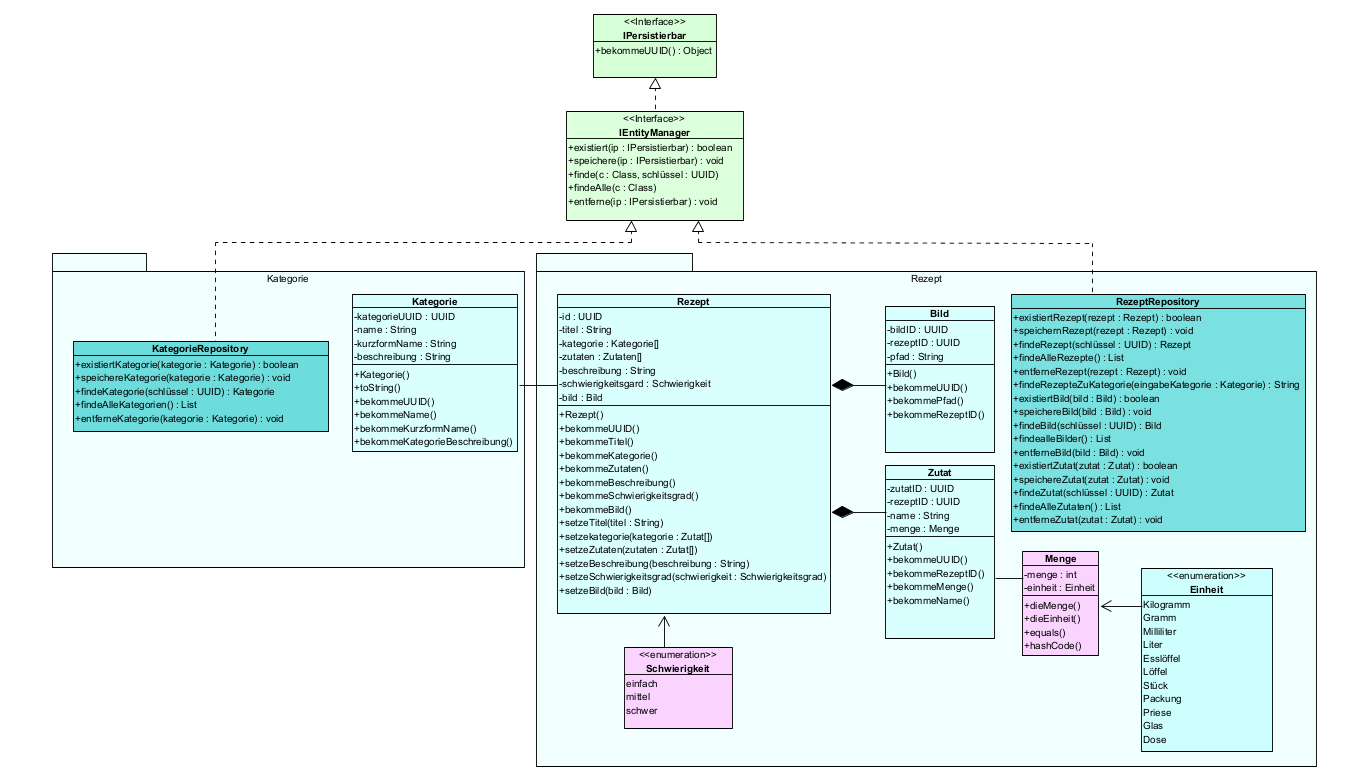
\includegraphics[width=0.90\textwidth]{Bilder/DomainCode-UML.png} 
	\caption{UML-Diagramm Domain Code Schicht}
	\label{fig:DomainCodeUML}
\end{figure}

\section{Schicht 1: Adapters}
Die Adapters-Schicht in Clean Architecture stellt die Schnittstelle zwischen der Anwendung und externen Systemen dar. Sie ermöglicht die Kommunikation der Anwendung mit der Umgebung und besteht aus Adaptern, die dafür verantwortlich sind, die Daten von der Anwendung in eine Form zu konvertieren, die von den externen Systemen verarbeitet werden kann und umgekehrt. In unserer Anwendung befinden sich in der Adapters-Schicht die Funktionalität für die Speicherung und für die GUI. 

Der EntityManager, welcher für die Datenhaltung zuständig ist, implementiert nun das Interface IEntityManager aus der Domain Code-Schicht (siehe \autoref{DI} Dependency Inversion). Darüber hinaus befindet sich in dieser Schicht die Konvertierung der Daten, die für die Speicherung notwendig ist. In dieser Anwendung wurde sich für eine Speicherung der Daten in CSV-Dateien entschieden. Die CSV Funktionalitäten werden möglichst in die äußeren Schichten implementiert, um die Art der Speicherung austauschbar zu gestalten. 
Für die Konvertierung wurde der Ordner Datenpersistenz erstellt und das Interface ICSVPersistierbar erstellt. ICSVPersistierbar wird dazu genutzt, um sicherzustellen, dass die zugrunde liegenden persistierbaren Entitäten eine UUID zum Speichern sowie einen Kopf und Daten für die CSV Dateien bereitstellen. Außerdem befinden sich im Ordner zu jeder persistierbaren Entität des Domain Codes eine eigene Klasse, die dieses Interface implementiert und somit explizite Funktionalität zur Speicherung in CSV Dateien beinhaltet. 

Zusätzlich wurde der DataReader implementiert, der die Funktionalitäten zum Laden der Daten aus den CSV Dateien in den EntityManager und das Speichern in CSV Dateien beinhaltet. Hierfür erstellt der DataReader die Instanz des EntityManagers und ruf dann die Funktionalität des CSVReaders oder des CSVWriters auf, welche die Daten laden oder speichern. 

Um die Code-Qualität und Wartbarkeit zu verbessern, wurden die Funktionen, die zuvor in den GUI-Klassen enthalten waren, in separate Funktionen-Klassen ausgelagert. Diese Funktionen-Klassen sind nun Teil der Adapters-Schicht, die als Vermittler zwischen der Benutzeroberfläche und den Daten fungiert.


\section{Schicht 0: Plugins}
In der Clean Architecture sind Plugins optional einsetzbare Komponenten, die von der Kernanwendung getrennt sind und über Schnittstellen integriert werden können. Sie ermöglichen es, die Anwendung um zusätzliche Funktionen oder Integrationsmöglichkeiten zu erweitern, ohne die Kernanwendung selbst zu verändern. In unserer Anwendung haben wir die Plugins in Plugins und Plugins-Main aufgeteilt.
In den Plugins sind alle GUI-Klassen implementiert.
Die Plugins-Main Schicht beinhaltet die Main Methode zum Starten der App. In der Main-Methode wird die DataReader Instanz instanziiert und die Daten aus den CSV Dateien geladen, bevor die Startseite gestartet wird. Da die darunter liegenden Schichten aufgrund der Dependency Rule dann nicht mehr auf den DataReader und somit auch nicht auf den EntityManager zugreifen könnten, wird die Instanz des DataReaders an die darunter liegenden Schichten beim Aufruf weitergegeben.


\section{Dependency Inversion}
\label{DI}
In der ursprünglichen Architektur haben Repositories innerhalb der Domain-Schicht den EntityManager aus der Adapters-Schicht aufgerufen. Dies verstieß gegen das Prinzip der Dependency Rule, das besagt, dass Abhängigkeiten immer von innen nach außen gerichtet sein sollten.

Um dieses Problem zu beheben, werden die Prinzipien der Dependency Inversion und Injection eingesetzt, um sicherzustellen, dass der EntityManager in der Domain-Schicht aufgerufen werden kann, ohne die Abhängigkeiten zwischen den Schichten zu verletzen.
Zu diesem Zweck wird das Interface IEntityManager, in der Domain-Schicht erstellt, welches die Methoden des EntityManager beinhaltet. Der EntityManager selbst wird in die Adapters-Schicht verschoben und implementiert dieses Interface. Um sicherzustellen, dass die Repositories auf den EntityManager zugreifen können, wird beim Aufruf des Repositories ein EntityManager Objekt übergeben. Da der EntityManager nun als IEntityManager-Typ im Repository-Code deklariert ist, kann er auch in der Domain-Schicht aufgerufen werden, ohne die Dependency Rule zu verletzen. Außerdem war hierbei wichtig, dass Entities in Domain Schicht IPersistierbar implementieren, da dies in EntityManager vorausgesetzt wird. 

Durch die Verwendung von Dependency Inversion und Injection wird die Abhängigkeit zwischen der Domain-Schicht und der Adapters-Schicht umgekehrt, sodass die Domain-Schicht unabhängig von der Adapters-Schicht bleibt. Dies verbessert die Flexibilität und Wartbarkeit der Anwendung und ermöglicht es, Komponenten einfach auszutauschen oder zu erweitern, ohne dass dies Auswirkungen auf andere Schichten hat.


